\subsection{Initial work}
This iteration did not consist of any development, that begins in iteration 1. It consisted mainly of research and some design work. But most importantly it included writing the stories for the project. 

Other smaller bits of work involved setting up a diary, a Trello board for documenting all the work and setting up the initial Git repository along with linking it to Github.
\subsubsection{Research}
Research was focussed on several areas, and some documents were produced from this research. The first area of research was on the frameworks available, after which Laravel was selected. Hosting options were also explored and a document discussing both of these was produced.

Some additional research was also completed on the Microsoft PowerPoint Add-In for the second part of the project. This was mainly to get a sense of the amount of work involved, and what language/ environments would be needed. This research did not go into much depth as further research will be undertaken when that part of the work is reached.
\subsubsection{Design}
The design work completed was a database design. This will be needed throughout the whole project so makes sense to write now, though it may be subject to significant changes. Figure \ref{fig:initial-er-diagram} is the ER diagram.

\begin{sidewaysfigure}
	\caption{Entity relationship digram for the initial database}
	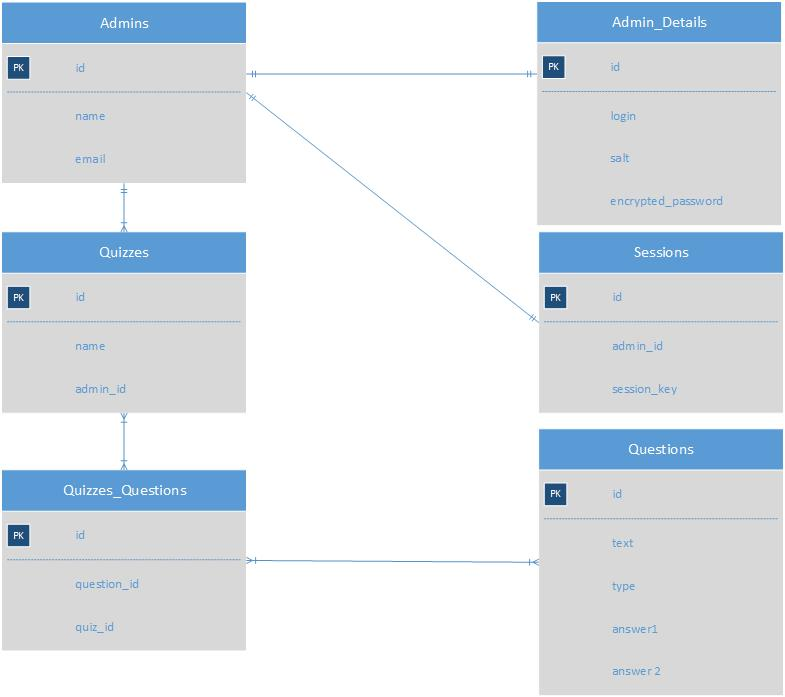
\includegraphics[width=\textwidth]{Chapter2/Iter-0/Initial-ERDiagram}
	\label{fig:initial-er-diagram}
\end{sidewaysfigure}

\subsubsection{Stories}
A list of stories was produced and written up in a separate document. These stories will be the basis of the project and act as the functional requirements for the evaluation at the end of development. TODO: list of stories in the appendix
\newpage